\documentclass[12pt, a4paper]{article}
 

\usepackage{geometry}
\usepackage{graphicx}
\usepackage{graphbox}
\usepackage{fullpage}
\usepackage{lmodern}
\usepackage{blindtext}
\usepackage{multicol}
\usepackage{enumitem}
\usepackage{amsmath}
\usepackage[table,dvipsnames]{xcolor}
\usepackage{titlesec}
\usepackage{caption}
\usepackage{float}
\usepackage{pgfplots}
\usepackage{pgfplotstable, tabularx}
\usepackage{booktabs}
\usepackage{tikz}
\usepackage{multicol}
\usepackage{cleveref}
\usepackage{siunitx}
\usepackage{tikzducks}
\usepackage{fancyhdr}
\usepackage{layout}
\usepackage{makecell}
\usepackage{pdfpages}

\usetikzlibrary{calc, shapes}

\geometry{margin=0.5in, bottom=0.6in, footskip=38pt}
\linespread{1.15}

\makeatletter
\global\let\tikz@ensure@dollar@catcode=\relax
\makeatother

\pagestyle{fancy}
\fancyhead{}
\fancyfoot{}
\fancyhf{}
\renewcommand{\headrulewidth}{0pt}
\renewcommand{\footrulewidth}{0pt}
\fancyfoot[C]{
        \shuffleducks{}
        
\begin{tikzpicture}[scale=0.4]
                \duck[signpost=\scalebox{0.6}{\thepage},\randomhead]
        \end{tikzpicture}
}

\crefname{figure}{Figure}{Figures}
\crefname{table}{Table}{Tables}
\crefname{equation}{Equation}{Equations}
\crefname{section}{Section}{Sections}

\pgfplotsset{compat=newest}
\pgfplotstableset{col sep=comma}

\captionsetup{justification=centering}

\setlength{\parindent}{0em}

\setcounter{tocdepth}{2}
\setcounter{secnumdepth}{2}

\newenvironment{Figure}
  {\par\medskip\noindent\minipage{\linewidth}\centering}
  {\endminipage\par\medskip}

\allowdisplaybreaks[2]

\begin{document}
    \thispagestyle{empty}
    
     \begin{tikzpicture}[overlay,remember picture]
        \node[at={($(current page.south east)$)},anchor=south east]{ \begin{tikzpicture}[scale=0.8]
        \tikzstyle{ct} = [draw,very thin,color=black];
        \tikzstyle{pf} = [fill=green];
        \path [pf] (0,1) -- (0,4) -- (1,4) -- (1,5) -- (2,5) -- (2,6) -- (3,6) -- (3,7) -- (4,7) -- (4,6) -- (7,6) -- (7,7) -- (8,7) -- (8,6) -- (9,6) -- (9,5) -- (10,5) -- (10,4) -- (11,4) -- (11,1) -- (10,1) -- (10,3) -- (9,3) -- (9,1) -- (8,1) -- (8,2) -- (3,2) -- (3,1) -- (2,1) -- (2,3) -- (1,3) -- (1,1) -- cycle;
        \path [pf] (3,7) -- (2,7) -- (2,8) -- (3,8) -- cycle;
        \path [pf] (8,7) -- (8,8) -- (9,8) -- (9,7) -- cycle;
        \path [pf] (3,1) -- (5,1) -- (5,0) -- (3,0) -- cycle;
        \path [pf] (8,1) -- (6,1) -- (6,0) -- (8,0) -- cycle;
        \path [fill=white] (3,4) -- (3,5) -- (4,5) -- (4,4) -- cycle;
        \path [fill=white] (7,4) -- (7,5) -- (8,5) -- (8,4) -- cycle;
        \path [ct] (0,1) -- (0,4) -- (1,4) -- (1,5) -- (2,5) -- (2,6) -- (3,6) -- (3,7) -- (4,7) -- (4,6) -- (7,6) -- (7,7) -- (8,7) -- (8,6) -- (9,6) -- (9,5) -- (10,5) -- (10,4) -- (11,4) -- (11,1) -- (10,1) -- (10,3) -- (9,3) -- (9,1) -- (8,1) -- (8,2) -- (3,2) -- (3,1) -- (2,1) -- (2,3) -- (1,3) -- (1,1) -- cycle;
        \path [ct] (3,7) -- (2,7) -- (2,8) -- (3,8) -- cycle;
        \path [ct] (8,7) -- (8,8) -- (9,8) -- (9,7) -- cycle;
        \path [ct] (3,1) -- (5,1) -- (5,0) -- (3,0) -- cycle;
        \path [ct] (8,1) -- (6,1) -- (6,0) -- (8,0) -- cycle;
        \path [ct] (3,4) -- (3,5) -- (4,5) -- (4,4) -- cycle;
        \path [ct] (7,4) -- (7,5) -- (8,5) -- (8,4) -- cycle;
        \end{tikzpicture}};
    \end{tikzpicture}
    \begin{tikzpicture}[overlay,remember picture]
        \begin{scope}
        \fill[blue!80] ($(current page.north east)+(-8,0)$) -- ($(current page.north west)+(5,0)$) -- ($(current page.north west)+(5,-7)$);
%         \node[regular polygon, regular polygon sides=6, fill=red!80, minimum size=12cm] at ($(current page.south east)+(-1,1)$) {};
%         \node[regular polygon, regular polygon sides=6, fill=orange!80, minimum size=10cm] at ($(current page.south east)+(-1,1)$) {};
%         \node[regular polygon, regular polygon sides=6, fill=yellow!80, minimum size=8cm] at ($(current page.south east)+(-1,1)$) {};
%         \node[regular polygon, regular polygon sides=6, fill=green!80, minimum size=6cm] at ($(current page.south east)+(-1,1)$) {};
%         \node[regular polygon, regular polygon sides=6, fill=blue!80, minimum size=4cm] at ($(current page.south east)+(-1,1)$) {};
%         \node[regular polygon, regular polygon sides=6, fill=purple!80, minimum size=2cm] at ($(current page.south east)+(-1,1)$) {};
        \end{scope}
        \begin{scope}
        \fill[red!80] ($(current page.north west)+(5,0)$) rectangle ($(current page.south west)$);
        \end{scope}

        \draw[ultra thick,gray] ($(current page.north east)+(-3.5,-0.5)$) -- ++(0,-3cm) 
            node[midway,left=0.25cm,text width=10cm, align=right, black!75]{{\fontsize{25}{30}\selectfont\textbf{ELEC3371}\\[15pt]\textbf{University Of New Haven}}}
            node[midway,right=0.25cm,text width=6cm,align=left,orange]{
\includegraphics[width=3cm]{univseal.png}};

        \node[anchor=north west, align=left, text width=25cm] at ($(current page.west)+(5,2)$) {{\fontsize{60}{72}\selectfont\textbf{Project 8:}\\[15pt]Space Invaders}};
        
        \hyphenpenalty=10000 
        \node[anchor=north west, align=left, text width=25cm] at ($(current page.west)+(5,-4)$) {{\fontsize{32}{42}\selectfont\textcolor{orange}{Written by Jamal Bouajjaj}}};
        \node[anchor=north west, align=left, text width=15cm] at ($(current page.west)+(5,-5.5)$) {{\fontsize{32}{42}\selectfont\textcolor{brown}{With the help of Cooper Biancur, Kosal C Vickcheka, and Akhil Manukonda}}};
        \node[anchor=north west, align=left, text width=25cm] at ($(current page.west)+(5,-9)$) {{\fontsize{35}{42}\selectfont 2020-12-14}};
    \end{tikzpicture}
    \clearpage
    
    \thispagestyle{empty}
    \hspace{0pt}
    \vfill
    \section*{\centering Abstract}
    \begin{center}
    \hyphenpenalty=10000 
    This project's goal was to recreate the legendary game \textit{Space Invaders} using an STM32F107 in a MikroE V7 development board for ARM. The board features a 320x240 LCD, a buzzer, a joystick, an analog potentiometer, and an EEPROM which were all utilized for this project. The game features a main menu, in which either the game can be started or an options menu can be selected. The main menu also shows the high score and it's player's name. The game offsets settings like enabling or disabling the protective walls, changing the bullet size, enabling or disabling sound, and more. The game starts with an entry animation of the aliens from the main menu. After, the game is yours to play. Your task is to kill all aliens without beign killed yourself. You can use the on-board potentiometer to speed up or slow down the game to your liking. 
    \end{center}
    \vfill
    \hspace{0pt}

    \newpage
    \thispagestyle{empty}
    \tableofcontents
    \newpage
    
    \pagenumbering{arabic}
    \section{Intro}
    As discussed in the Abstract, the goal of this project is to re-create the game \textit{Space Invaders}. Unfortunately due to time and the way I implemented it, there are some derivations from the original game. For example, due to the size I originally set out to create the aliens, I only have 15 of them. This could be changed tough as discussed in \cref{conc:future}.
    
    \section{Hardware} \label{sec:hardware}
    The hardware for this project is all centered around the MikroE for ARM V7 development board. There are 7 main components that we care about tough, which are the microcontroller, LCD, buzzer, EEPROM, a button, a potentiometer, and the joystick. An overall schematic of the components that matter for this project are shown bellow:
    \begin{Figure}\centering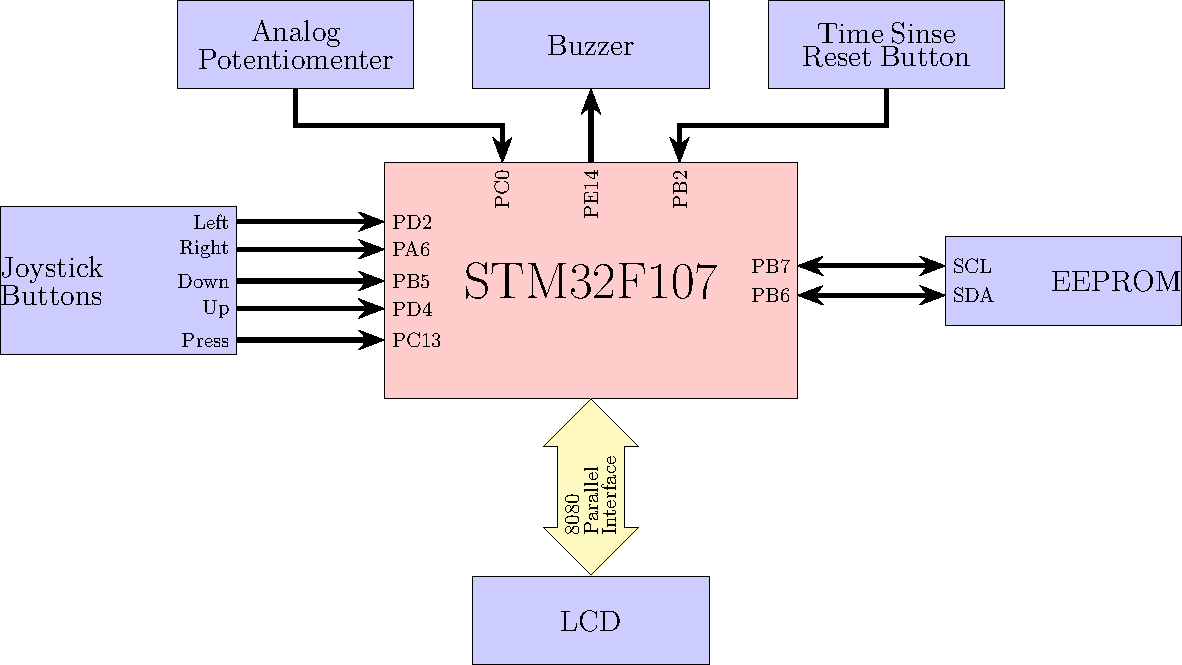
\includegraphics[width=0.95\textwidth]{TikzDrawings/schematic.pdf}\captionof{figure}{Overall Program's Hardware Layout and Wiring}\end{Figure}
    
    \subsection{LCD}
    The LCD on the development board is one with an ILI9341 driver IC (the chip that controls the panel's output). This chip is interfaced with the microcontroller with an 8080 8-bit parallel interface. The different wires connecting the 2 goes as follows:
    
    While one might think that because it's parallel it would be faster, that isn't quite the case. If the LCD was running off of SPI, we will be able to store a buffer in the microcontroller then have a DMA send it our, freeing the CPU to do other tasks (like perhaps fetching more data to be sent or dealing with the game). 
    
    Unfortunately the LCD doesn't have a double-buffer, so if a image was to be displayed, you will see the display change as the internal display RAM is updated. If it was double-buffered, we would see an instantaneous change when we latch the data from the first buffer to the second.
    
    \subsection{EEPROM} \label{hardware:eeprom}
    The EEPROM on the development board is an 24AA01 EEPROM by Microchip. The EEPROM is organized as one block of 120x8-bit memory. It's interfaced to the microcontroller with the $I^2C$ protocol. 
    
    One interesting thing about the EEPROM that isn't mentioned too well in it's datasheet is it's page size of 8-bytes. This is important if we want to update 8 bytes at once, as the starting address needs to be aligned in 8-byte chunks. This was learned the hard way, as talked about in \cref{conc:strugle}.
    
    \section{Software - Overview}
    \subsection{Layers}
    The software is designed around 3 different layers. Each layer only interacts with the layer above it and below it, for the most part. The exception to this in the program is the Interrupt Handlers in the \textit{LL Drivers} layers, which partially directly communicates with the \textit{Game Logic} layer. This is equivalent to how modern operating systems work, where the kernel only interfaces between the OS and the hardware, and the OS doesn't directly interface to the hardware. The software layers for this program are show below:
    \begin{Figure}\centering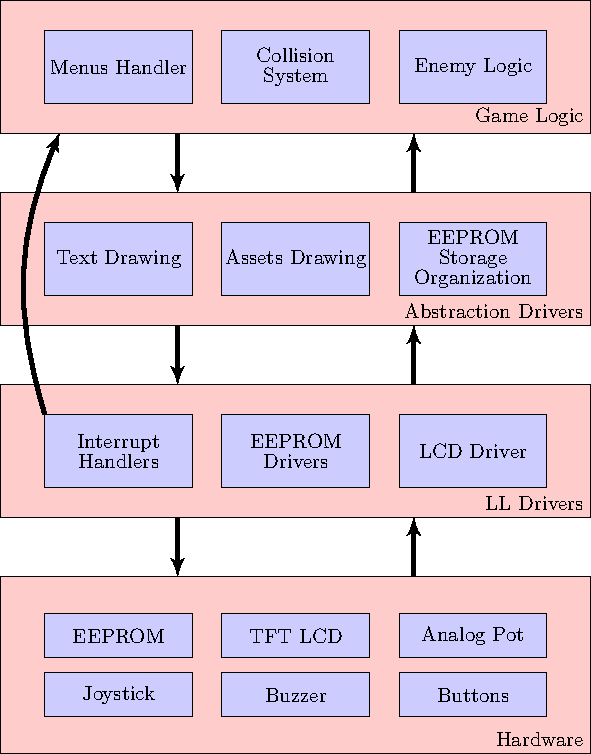
\includegraphics[width=0.75\textwidth]{TikzDrawings/highlevelorg.pdf}\captionof{figure}{Program's Layers}\end{Figure}
    On the bottom is the hardware layer, which isn't actually code but just the hardware talked about in \cref{sec:hardware}. 
    The layer above it is the Low-Level Drivers. This layer of code interfaces with the hardware, and opens up basic functions, like a function to write to the EEPROM or to initialize the LCD. This layer also includes all interrupt handlers. 
    The next layers is the Abstraction Drivers. This layer of code includes functions which abstract the low-level drivers to fit the needs of the Game Logic, which makes developing that layer much easier. Functions like \textit{movePlayerLeft}, \textit{moveAlienDown}, and \textit{displayText} are included in this layer.
    The top-most layer of this program is the Game Logic. Unlike what the name suggest, this does more than just game logic (I couldn't come up with a better name for this layer). This layer handles like like the different screen, the settings and main menu, and of course the actual game itself. 
    
    \subsection{States} \label{soft:over:states}
    This software comprises of 4 "States". A state is just a part of the program which runs forever until some event occurs. Think of it as a block in a state machine. The following diagram demonstrates the 4 states, and which other states they are able to go into:
    \begin{Figure}\centering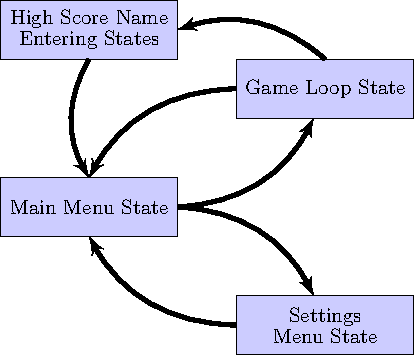
\includegraphics[width=0.75\textwidth]{TikzDrawings/gameloops.pdf}\captionof{figure}{Program's Loops}\end{Figure}
    The 4 states, as they are integral to the structure of this program, is described in details in \cref{sec:states}
    
    \subsection{Files Breakdown}
    As this project is massive compared to previous ones, multiple files were used to build the program. The table below describes each file or directory and gives a brief explanation as to why it's there (from the project's root perspective):
    \begin{table}[H]\centering\begin{tabularx}{\textwidth}{|l|X|} \hline \rowcolor[HTML]{FFCCC9} 
    \bfseries Folder/File(s) & \bfseries Description \\ \hline
    Driver/*        &   All Low Level and CMSIS drivers by ST.    \\ \hline
    Inc/*        &   Header files for \textit{main.c} and \textit{it.c}.  \\ \hline
    Startup/startup\_stm32f107vctx.s         &   The startup assembly file, generated by STM32CubeIDE.       \\ \hline
    Libraries/SDcard/* & Library for the SDcard. Not used in this project right now, is there when I played around with playing music.    \\ \hline
    Libraries/24AA01.*      & Driver for the EEPROM. \\ \hline
    Libraries/LCD.*      & Driver for the LCD. \\ \hline
    Libraries/VS1053.*      & Driver for the VS1053 audio IC. Not used in this project right now, is there when I played around with playing music.\\ \hline
    Libraries/vars.*      & Global variables and struct definitions. \\ \hline
    Src/main.c      & The main program. \\ \hline
    Src/it.c      & All interrupt calls. \\ \hline
    Src/*others*.c      & Other C files, generated by STM32CubeIDE.       \  \\ \hline
    \end{tabularx}
    \caption{Files and Folder description of Program}
    \end{table}
    
    \section{Software States} \label{sec:states}
    As mentioned in \cref{soft:over:states}, the program is comprised of 4 "States" which this section will go over and describe.
    \subsection{Main Menu States}
    This loop is the first one that gets called when the program is started up. It includes a title, some moving aliens (which will be used during the transition to the game loop state as discussed later), the player, the high score and it's player, the time since death or reset, and 2 options.
    
    When this state gets loaded it, it retrieves the top score and the top score player from the EEPROM, and displays them. It also draws 5 aliens and player in a desired position. Next 2 options are shown: \textit{"Start Game"} and \textit{"Game Settings"}. Then, this state goes inside an infinite loop which moves the 5 aliens left and right. Everytime the aliens hit the arbitrary right boundary, the players "face" changes. This loop also checks if we pressed PB2 in order to switch between showing us the time since death or since reset. It also checks if we are exiting this state to another one, then goes thru a transition function for the 2 possible states it's able to go to, then exits out of this loop. 
    
    There are several functions related to this state in which the interrupt handlers call. One of them is called when we press the up and down joystick buttons, which will simply change which of the 2 options we have selected. Another one gets called when we press on the joystick, which changes a variable to let the state's infinite loop know if we are transitioning and to which other state so it could execute the right transition function, then exit out of the screen. The last interrupt-called function is called when the reset and death counter (talked about in \cref{soft:comp:counter}), which updates either the death or reset counter on-screen, depending on which one was selected by PB2.
    
    As mentioned, when we press on the joystick and it's interrupt function gets called, it changes a variable which this state's infinite loop checks for. If it's not 0, it calls a transition function depending on which state we are transitioning to. If it's the settings menu, it simply clears the screen, that's it. If it's the game loop state tough, it gets a little interesting. First, it moves the 5 aliens down by a certain amount. Then it moves them left or right depending on where they currently are until they are centered. Then, 2 5-rows of aliens gets created and transitioned in, having the first row move from the left side of the screen, and the second row from the right side of the screen. The result is 3 rows of 5 aliens per row at the end, which the game will start out with.
    
    \subsection{Settings Menu States}
    This state is for the user to select different game settings. This state initializes itself by simply drawing out the different options. Then inside it's infinite loop, it just checks if we need to exit out of this state and go back to the main state, which it does by simply clearing the screen. 
    
    There are 4 options in this game which goes as follows:
    \begin{itemize}[noitemsep]
     \item \textit{Walls?} $\rightarrow$ Determines if the game will have protective walls.
     \item \textit{Bullet Size} $\rightarrow$ Determines the width of the bullet, wither tiny or large.
     \item \textit{Sound On?} $\rightarrow$ Determines if the game will have any sounds at all.
     \item \textit{Infinite Walls} $\rightarrow$ Determines if the protective walls will have infinite health.
    \end{itemize}

    There are 3 interrupt-called functions related to this state. One of those gets called when the up or down joystick button gets pressed, which changes which option we are currently on. The other function gets called when we press the right or left joystick button gets pressed, which changes the setting and updates which one is highlighted or not. The last interrupt-driven function gets called when we press the joystick, which only does something if we are on the last option (the \textit{"Go Back"} option) that changes a variable to let the infinite loop know we need to exit out of this state.
    
    \subsection{Game Loop States} \label{subsec:loop:game}
    This is by far the most important state in this program, as it handles the game itself. When the state is initially called, it assumes the aliens are in the right place, as the only state that could call this one is the \textit{Main Loop} state, which places the aliens at the right position before changing to states. If the protection walls are enabled, it initialize them with their abstraction driver function. It does clears and sets a bunch of variables and arrays before going inside it's infinite loop.
    
    In this state's infinite loop, that's where the game logic occurs. At the end of this loop, before looping thru again, there is a small delay. This means that the game logic is executed every $x$ milliseconds, which could be tough of as the game's update cycle (just like Minecraft updates once every 20 ticks). At the start of the loop, the ADC is triggered by software to measure the output of the pot (important for later). Then a function which moves the aliens is called only if we are not \textit{God mode}. That function moves all aliens left$\rightarrow$down$\rightarrow$right$\rightarrow$down, then left again in a cycle. Then we iterate thru all available player's bullet's array and check if they are alive (meaning it's on screen and should be moving). If so, we move the bullet up and check for collision against any alien, wall or if the bullet is on top of the screen. If the bullet is on top of the screen, we simply kill it. If it collided with a protective wall, we kill the bullet and add damage to the wall. If it collided with an alien, we kill both the alien and the bullet, decrement the alien count, and add a score as determined by \cref{eq:score} and update the score shown. Then after that, we check for all alien's projectile array. If a projectile isn't alive, if we're not in \textit{God mode} we create one and play a tune by a chance given by \cref{eq:alienbulletchance}. If a bullet is alive tough (meaning an alien shot back), we move it down and check for collision against the player and the protective walls. If it hits a protective walls, we kill the projectile and add damage to the walls. If it hits a player, it ends the loop and goes to a \textit{Game Over} screen that is discussed later. Then the loop checks if the aliens hit the bottom of the screen where the player is, which also ends with a \textit{Game Over} screen. The loop then checks on the number of aliens, and if that's zero we end the game with a \textit{You Win} screen that is discussed later. After, right before we delay the game logic, it retrieves the ADC value that we triggered at the start of the loop and maps the ADC value to a value between $10$ and $200$, which corresponds to the game delay in milliseconds.
    
    When the game has ended, it shows either a \textit{Game Over} or a \textit{You Win} screen depending if we won it lost. It also plays a tune depending if we lost or won. Then, it checks the game's score vs the high score, which if the game score is higher it goes into the \textit{High Score Name Entering} state (\cref{subsec:loop:score}). Either way, right before it goes back to the \textit{Main Menu} state it clears the screen and resets the "time-since-death" counter back down to 0.
    
    There are 2 interrupt-called functions related to this state. One of them gets called when the joystick is pressed, which simply initialize at bullet at the player's location. Before it does that tough, it checks if we entered the right combination for \textit{God mode}. The other function gets called when we press the up or down joystick buttons. They are used to enter the combination for \textit{God mode}, which the right combination is stored in an array. This function indexes a variable by 1 only if the right joystick is pressed for the current combination key, and resets it if not. 
    
    The combination of the 2 interrupt-called functions as far as \textit{God mode} is considered is that the right combination must be entered, then the joystick must be pressed in order to go into \textit{God mode}.
    
    The player's movement is handled by the interrupts directly as talked about in \cref{soft:comp:pla}.
    
    
    \subsection{High Score Name Entering State} \label{subsec:loop:score}
    This loop only gets called when there is a new high score. This loop allows the player to enter a name. The name selection is done by changing 8 characters shown on the display. After setup, the only thing happening inside this loop's infinite while statement is checking if we are done with this loop to give control back to the calling function (to eventually go back to the Main Menu loop). 
    
    This loop has 3 associated functions which gets called by interrupt handlers. One gets called when the up or down joystick button is pressed, which increments or decrements the letter shown on screen for the selected character (A partial bug in this function exists, talked about in \cref{conc:sucandbugs}). Another one gets called when the left or right joystick button is pressed, which simply changes which character we are manipulating. The last functions gets called when the joystick is pushed, which changes a flag to allow the Loop's while loop to exit.
    
    \section{Software Components}
    \subsection{LCD}\label{soft:comp:lcd}
    While writing my own library for the LCD, as this game is mostly single-color I've decided to make a custom function which simply draws an image on the screen. The data for the image is simply an array of bytes, in which each bit represents if the pixel is on or off. This array is generated by \cref{python:oncolor}. There is also a "backportch" and "frontporch" feature. This allows the function to clear the space beforehand and afterwards, allowing for easy scrolling/movement functionality. 
    
    A high level function handles drawing text. It does this by drawing a black and white image as we just described, with a font's black and white image array shifted over by a certain amount (that amount stored in another array). Then per character it offsets the x position by 2 plus the width of the drawn character (stored in another array).
    \subsection{EEPROM Storage}
    The EEPROM is organized to take advantage of the page write functionality of the 24AA01 IC. That is why the high score's name is limited to 8 characters, and why it start at address \textit{0x08}. Also 8 characters should be sufficient I think. A graphic showing how the memory is organized is shown bellow:
    \begin{Figure}\centering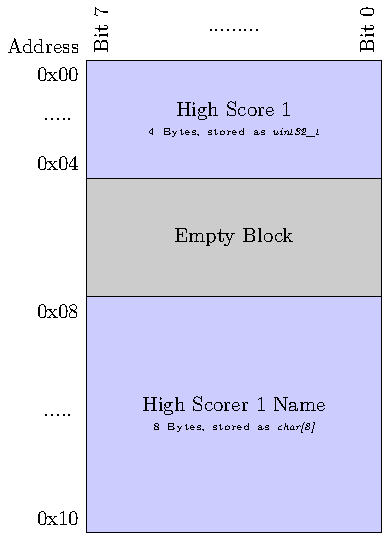
\includegraphics[width=0.75\textwidth]{TikzDrawings/eeprom.pdf}\captionof{figure}{EEPROM Memory Organization}\end{Figure}
    \subsection{Buzzer}
    The buzzer itself is controlled by 1 Timer: Timer 1. Instead of what I did on my last Project, I instead opted to use the Timer's PWM function. The buzzer is on PE14, which was controlled by Timer1's channel 4 output if remapped. Before Timer 1 is started, the timer's \textit{ARR} is updated according to \cref{eq:arrcalc}, and \textit{CCR4} is half of \textit{ARR}(so that the duty cycle is 50\%).
    
    There is another Timer in play tough, Timer 3. The purpose of that timer is simply to stop Timer 1 when it interrupts. The reason for this is because you could start up both Timer3 and Timer1, and have the sound automatically cut off after a certain time asynchronously. This allows for 1 function that the rest of the program could call which, if a sound isn't currently playing, plays a tune of $x$ frequency for $x$ milliseconds. For this program, that function is \textit{start\_beeper()}.
    \subsection{ADC and Pot}
    An Analog-To-Digital Converter built into the microcontroller was used to determine the game delay mentioned in \cref{subsec:loop:game}. We had PC0 be the ADC input, in which PC0 is connected to a potentiometer. This input corresponds to channel 10 on the ADC. ADC1 was the peripheral used, set to only start a measurement when triggered by software. 
    \subsection{Reset and Death Counter} \label{soft:comp:counter}
    The time since death and reset counters are 2 integers increment once a second. This is done thru Timer 2, which is set up to interrupt once a second as long as the program is running. Inside that interrupt, it simply increments both counters and calls on the \textit{Main Menu}'s state \textit{menuUpdateTimeShown()} function to update the time shown if we are in that state.
    \subsection{Player Movement} \label{soft:comp:pla}
    The player's movement, unlike all other parts of this program, is handled directly by the interrupt handlers if we're in the \textit{Main Menu} or \textit{Game Loop} states. It moves the player by starting a timer (Timer 7), in which everytime the timer is triggered it moves the player 1 space to the right or left depending on which joystick button we pressed (left or right). It stops movement by simply stopping that timer. This is kind of messy, as ideally the interrupt handlers will call a function that is part of the \textit{Game Logic} layer to handle moving the player. This can be changed tough as mentioned in \cref{conc:future}
    
    \section{Python Programs}
    Some custom Python programs were used to generated the font and image data.
    \subsection{One Color Image} \label{python:oncolor}
    This Python program (ILI9341\_OneColor.py) generated an array of bytes, in which each bit represents if the pixel is on or off. The input argument to this program is an image file, in which all pixels to be lit up are black and ones that aren't white in the image.
    \subsection{Font Generator}
    This Python program (char\_img\_generator.py) generated 3 arrays to draw out the font as described in \cref{soft:comp:lcd}. The first array is an array of all character's (between ! and $\sim$ in ASCII) B\&W array in a single dimension array. Then it generates an offset array, so that the program is able to know where each character's black and white array starts in the large B\&W array generated. Last, it generates a width array, storing the width of each character. The text is created from a font file, so it's add done automatically. 
    
    \section{Results and Conclusion}
    \subsection{Trials} \label{conc:strugle}
    As mentioned in \cref{hardware:eeprom}, one thing that was causing a major bug is the page size. This is important as in my program I'm using the page write functionality. I did not realize at the time of the page size allocation (where it starts at every 8-bytes). If the EEPROM gets tht end of a page during a page write command, it will just go back to the start of that page. This is what I was getting weird numbers and names when I started storing the name at address \textit{0x04}. Luckly my logic analyzer quickly lead to the program, as I was able to visually see what packets are sent across and noticed pattern when reading the data at certain addresses. It also help me assure that my low-level driver for the EEPROM is functional. 
    
    Another issues that I had to deal with is debouncing. Because the inputs are interrupted, if there is a debounce on the joystick buttons the interrupt will trigger again. A solution for this dilemma that works well enough is to add a debounce delay before clearing the EXTI's interrupt pending flag. That way, even if the interrupt "triggers" again during the delay, it wont execute as the pending flag will be cleared. Another solution for debouncing is to add capacitors in parallel with the buttons, slowing their rise time and hopefully eliminate debouncing. 
    
    \subsection{Success?} \label{conc:sucandbugs}
    At the end of the day, we have a fully functioning game. It may not be the same as the original \textit{Space Invaders}, but I'm contempt with it. 
    
    There are some bugs tough that I noticed after finalizing the game and couldn't change due to time. One of them is during the \textit{High Score Name Entering} state, which there is no option to enter a space/empty character, uppercase letters, or number, only lower case letters. Another bug is in the transition between the \textit{Main Menu} and the \textit{Game Loop} state, which if the aliens are perfectly centered when the transition is called it will forever move the aliens right with on end.
    
    \subsection{Future Work} \label{conc:future}
    One of the first things I would do if I was to go back to this project is to fix the bugs mentioned in the subsection above. 
    
    Another things I would change about this project is having some numbers hardcoded (like player's width) by defined with a preprocessor \textit{\#define}. That would make it much easier in the future if something like the player's width needed to be changed without diving looking for it everywhere (especially as this is a relatively large project). 
    
    I would also remove the code inside the interrupt handlers which move the player and move them to be part of the \textit{Main Menu} and \textit{Game State}, and have the interrupt handlers call those respective functions if we are in that state. 
    
    As for features, I want to add the option to have multiple pages of settings, as well as add other options like the player's face during gameplay and other fun stuff. I would also add multiple alien's faces, which should be easy to do. I would also expand the program to have another high score player and score stored on the EEPROM (second place).
    
    \subsection{Appendix}
    The following equations were used throughout the program:
    \begin{gather}
     \label{eq:arrcalc} ARR = \frac{10000}{f}\\
     \label{eq:score} \text{Score} = 100 + rand(0\rightarrow 100) \\
     \label{eq:alienbulletchance} \text{Chance of Alien shooting back} = rand(0\rightarrow 200)
    \end{gather}
    
    The code is too large to add to the Appendix. If you would like a copy of that, as well as any other files used to make the project (including this report's .tex file), feel free to contact me at \textit{jboua1@unh.newhaven.edu} for such request.
    
    
\end{document}
